\chapter{Implementación del sistema}\label{sec:Implementacion}

\section{Adquisición}


En la adquisición de señales EMG hay que tener en cuenta un correcto acondicionamiento tanto como de la piel como del sistema.


\subsection{Preparación de la piel} \label{sec:Preparaciondelapiel}
 Es necesario a la hora de obtener señales EMG una correcta preparación de la piel dónde vamos a colocar los electrodos; de forma que la calidad de la señal obtenida sea la mejor posible. Para este propósito es recomendable usar un gel abrasivo o alcohol tanto para eliminar las células muertas de la piel como para reducir la sequedad de la misma. Tras la correcta limpieza con un paño suave se asegura que la zona quede totalmente limpia y seca. \newline
\subsection{Los electrodos} \label{sec:Loselectrodos}

Para ello se usan 3 electrodos  (2 y uno de referencia) que se colocan directamente sobre la piel y son capaces de captar la actividad bioeléctrica. La ubicación de los electrodos va a influir directamente sobre la calidad de las señales obtenidas; una correcta colocación sería en paralelo a las fibras musculares, en la zona central del músculo del que queramos obtener la actividad eléctrica. Estos deberán estar separados de 1 a 2 cm y el de referencia deberá estar colocado en un sitio dónde sepamos que la actividad será minima. En los tendones y el borde del músculo las fibras musculares se vuelven más delgadas y pequeñas por lo que son el sitio ideal para colocar el electrodo de referencia. 

Antes de colocar los electrodos se puede usar una pasta conductiva que mejora considerablemente la captación de estos de las señales.\newline

\begin{figure}[H]
	\center
	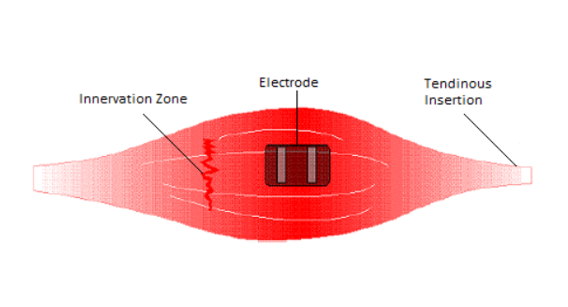
\includegraphics[scale=0.8]{imagenes/Implementaciondelsistema/electrodo.png}
	\caption{Posición de los electrodos}
	\label{fig:Posicion}
\end{figure}

\subsection{Captación de señales}

En la captación por lo tanto de señales EMG, con lo visto en \ref{sec:Preparaciondelapiel} y \ref{sec:Loselectrodos} tendríamos que definir el músculo que va a hacer de instrumento de control para el sistema. Se plantea la idea de usar un músculo del antebrazo por la facilidad para la colocación de los electrodos, así como a la hora de descriminar los distintos movimientos que nos van a permitir el control del sistema. Un correcto sitio sería con los 2 electrodos en la parte central y el de referencia en el codo que es un punto neutro.\newline 

El músculo flexor del carpo (figura \ref{fig:flexor}) será  el que eligiremos debido a su posición central, ya que permite contraerlo y relajarlo con facilidad. \newline Por lo tanto este será el músculo sobre el cual vamos a colocar los electrodos para realizar la toma de señales y empezar a discriminar los distintos movimientos.  

\begin{figure}[H]
	\center
	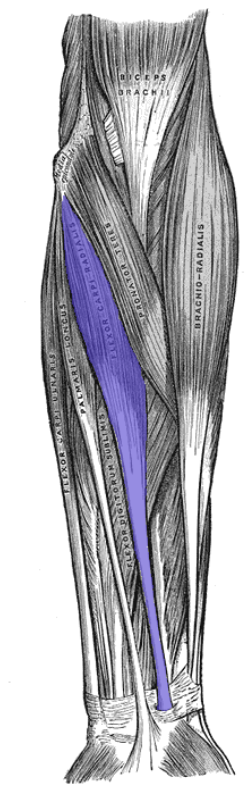
\includegraphics[scale=0.5]{imagenes/Implementaciondelsistema/flexor.png}
	\caption{Músculo flexor del carpo en el antebrazo}
	\label{fig:flexor}
\end{figure}


 las señales EMG de entrenamiento, que mediante Bluethooth son enviadas al ordenador en tiempo real y vistas en el software OpenSignals. Desde que ponemos en marcha el programa hasta que lo paramos las señales EMG captadas con los electrodos se pueden ver en el mismo programa,y elegir el rango de tiempo que queremos guardar. Estas señales guardadas en el ordenador son procesadas en Matlab para flitrar el rango que nos interesa de frecuencias, para eliminar el ruido y mediante umbrales discriminar si el movimiento es de más o menos intensidad. \newline
Una vez las señales son procesadas son enviadas mediante comunicación serie a la FPGA.



\section{Procesamiento en Matlab}